\documentclass[border=2pt,tikz]{standalone}
\usepackage{tikz}
\usepackage{amsmath}
\usepackage{amssymb}

\begin{document}

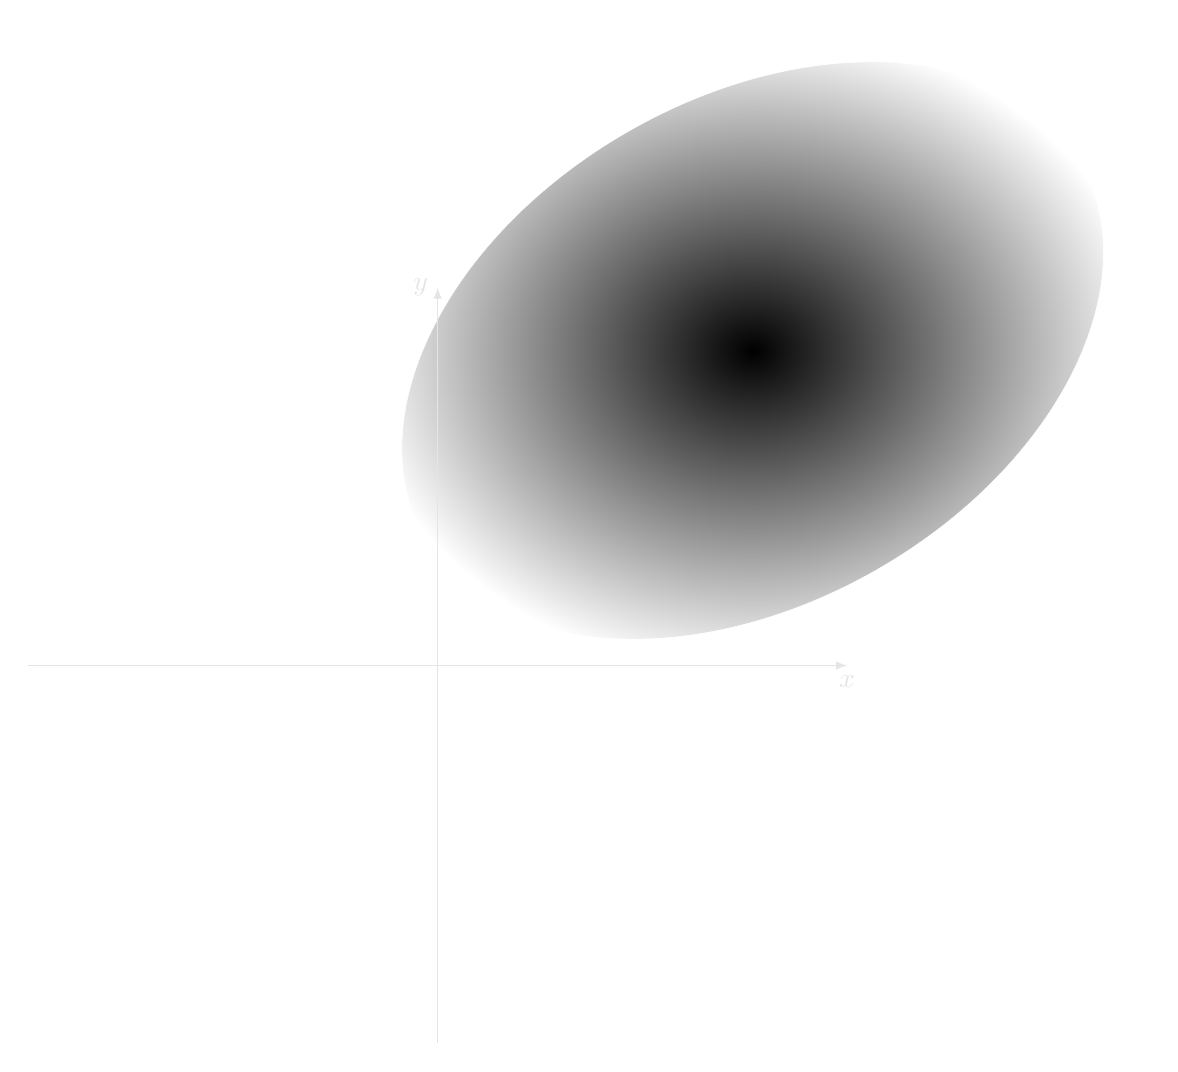
\begin{tikzpicture}[scale=4]

\begin{scope} [shift ={(1 ,1)}, rotate=30]

% FIXME: 程序有BUG,旋转之后灰度边缘不对。
\draw [very thin, lightgray!0, inner color=black!100, outer color=black!0] (0,0) ellipse (1.2 and 0.8);

% Draw x and y axis lines
%\draw [->,>=latex] (-1.3,0) -- (1.3,0) node [below] {$x^\prime$};
%\draw [->,>=latex] (0,-1.2) -- (0,1.2) node [left]  {$y^\prime$};

\end{scope}

% Draw x and y axis lines
\draw [->,>=latex, lightgray!40] (-1.3,0) -- (1.3,0) node [below] {$x$};
\draw [->,>=latex, lightgray!40] (0,-1.2) -- (0,1.2) node [left]  {$y$};

%\draw[very thick, ->,>=latex] ( 0.0, 0.0) --  node [above, rotate=45] {bias} (1.0,1.0);

\end{tikzpicture}

\end{document}

